\chapter*{Results}

\section{First analysis}

\begin{table}
    \caption{Instrument resolution function}
    \centering
    \begin{tabular}{|c|c|c|}
        \hline
        FWHM (ps) &  Shift (ps) & Intensity (\%) \\
        \hline
        213.3 & 0 & 80\\ 
        150 & -5 & 10\\ 
        267 & 17 & 10\\  
        \hline
    \end{tabular}
    \label{tab:irf}
\end{table}

\begin{figure}
    \centering
    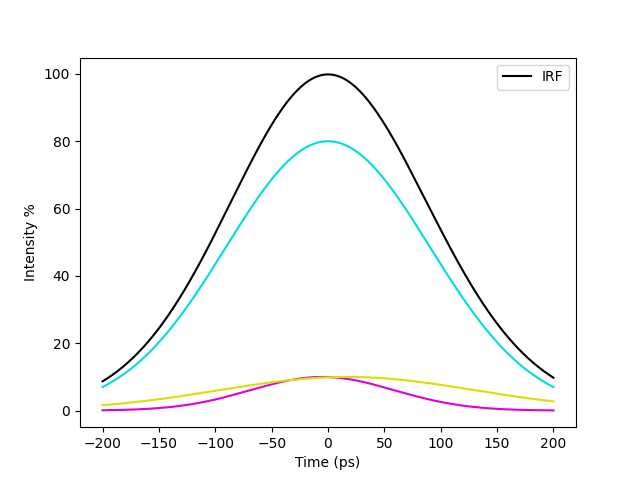
\includegraphics[width=0.8\textwidth]{Batch 3/regular IRF/irf.png}
    \caption{instrument resolution function}
    \label{fig:irf}
\end{figure}

Using PALSSIM, a series of spectra containing two positron lifetimes, $\tau_1$ and $\tau_2$, were generated with a three gaussian instrument resolution function (see Table \ref{tab:irf} and Figure \ref{fig:irf}). $\tau_1$ was kept fixed at 180ps and $\tau_2$ varied from 220-280ps, in 10ps intervals. For each value of $\tau_2$, three spectra were generated with the relative intensities of $\tau_1$ and $\tau_2$ set to 20\%-80\%, 50\%-50\% and 80\%-20\%. All the resulting spectra were then analyzed using PALSFIT, in order to evaluate how well the program could extract the two lifetimes, and their respective intensities, from each simulated spectrum.

In Figure \ref{fig:180-tau1}, we can observe how the values of $\tau_1$ outputted by the program change, as the simulated value of $\tau_2$ (on the horizontal axis) increases and the relative intensities (indicated by color and shape of marker) vary. Zooming in to the $\tau_2$ = 250-270ps range, we can see in Figure \ref{fig:180-tau1-zoomed} that, for these values in particular, PALSFIT struggles to determine $\tau_1$ in the 50-50 and 80-20 case. 

Unlike for $\tau_1$, where the simulated value of the lifetime is fixed, the simulated value of $\tau_2$ (our point of comparison) changes in between spectra. To make the data easier to visualize, rather than the fitted value of $\tau_2$, the difference between the result and the original is plotted instead (see Figure \ref{fig:180-tau2}). In the figure we can see that, aside from the 20-80 spectrum for $\tau_2$ = 220, the software performs better than for $\tau_1$.

The error bars represent the standard deviation of -- and thus the confidence of the program in -- the lifetimes. From them, we see two factors that affect the size of the bars. The first is the relative intensities of the two intensities. In fact, in Figure \ref{fig:180-tau1}, which plots $\tau_1$, the error bars are the smallest for the 80-20 data, where the shorter lifetime is more intense, and in Figure \ref{fig:180-tau2}, tracking $\tau_2$, the opposite is the case and we have the 20-80 data is most precise. Observing all the figures, we see the second factor: as the time interval between the two lifetimes increases, the size of the error bars decrease.

In Figures \ref{fig:180-2080} - \ref{fig:180-8020} the fitted intensities of the two lifetimes are plotted against simulated $\tau_2$, for each combination of simulated intensities. In the figures, we see that when the relative intensity of $\tau_2$ was greater or equal to $\tau_1$, then PALSFIT was able to calculate all the appropriate lifetime intensities. However, when the intensity of $\tau_2$ was set to 80\%, shown in Figure \ref{fig:180-2080}, the software was unable to output the correct intensities for the first two simulated values of $\tau_2$. Looking at our error bars, we can see the same relationship between their size and the lifetime separation mentioned earlier.

On the whole, PALSFIT seems to have performed well, but not perfectly. As the first lifetime, $\tau_1$, was kept constant at 180ps, the next step would be to change $\tau_1$ and see how that affects our results. 

\todo{expand paragraph}

\begin{figure}[p]
    \caption{}
    \centering
    \makebox[\linewidth][c]{
        \begin{subfigure}{0.7\textwidth}
        \centering
        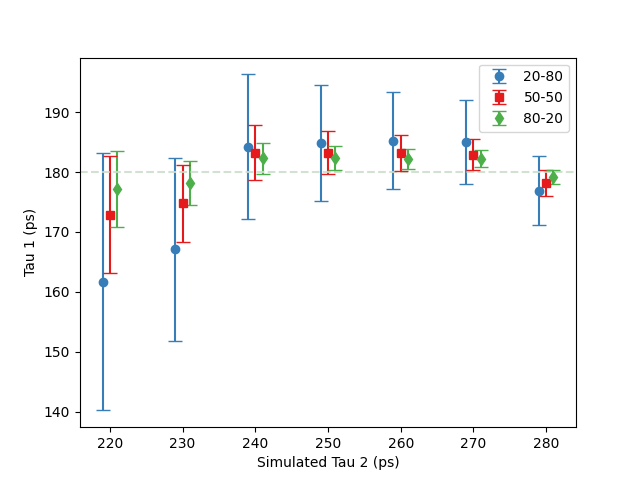
\includegraphics[width=0.95\linewidth]{Batch 1+2/t1.png}
        \caption{fixed $\tau_1 = 180ps$}
        \label{fig:180-tau1}
    \end{subfigure}
    \begin{subfigure}{0.7\textwidth}
        \centering
        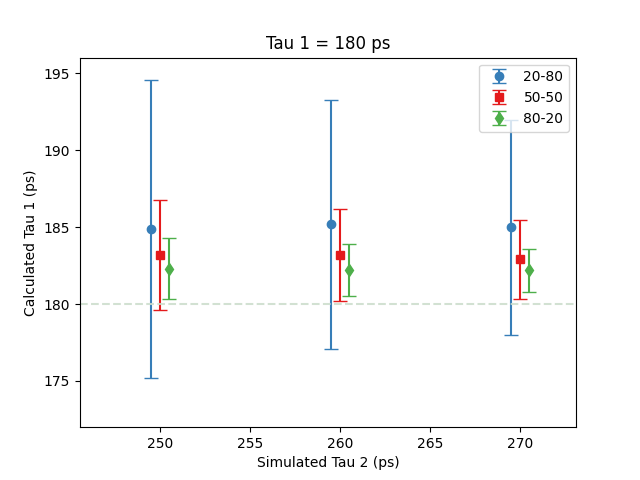
\includegraphics[width=.95\textwidth]{Batch 1+2/Tau1 stragglers.png}
        \caption{close-up $\tau_1 = 180ps$}
        \label{fig:180-tau1-zoomed}
    \end{subfigure}
    }
    \makebox[\linewidth][c]{
    \begin{subfigure}{0.7\textwidth}
        \centering
        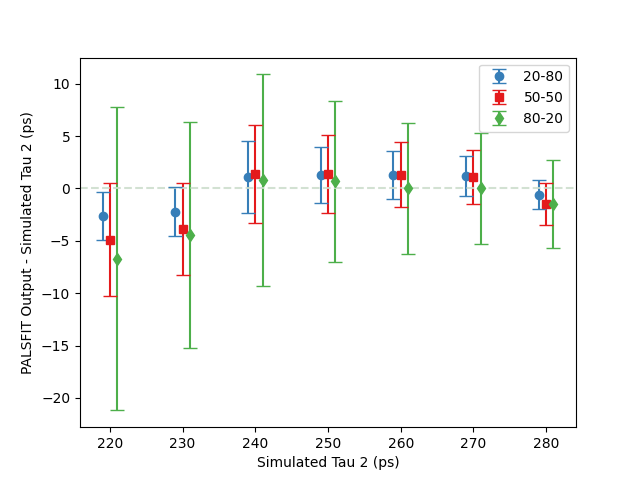
\includegraphics[width=.95\linewidth]{Batch 1+2/t2.png}
        \caption{$\tau_2$ difference}
        \label{fig:180-tau2}
    \end{subfigure}
    \begin{subfigure}{0.7\textwidth}
        \centering
        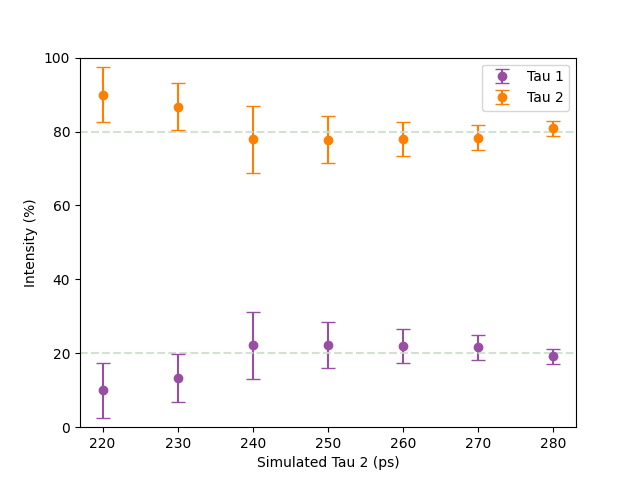
\includegraphics[width=.95\linewidth]{Batch 1+2/2080.png}
        \caption{$\tau_1 = 20\%, \tau_1 = 80\%$}
        \label{fig:180-2080}
    \end{subfigure}
    }
    \makebox[\linewidth][c]{
    \begin{subfigure}{.7\textwidth}
        \centering
        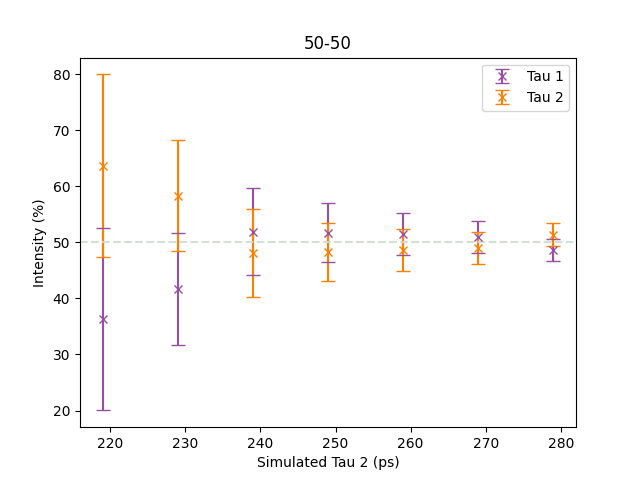
\includegraphics[width=0.95\linewidth]{Batch 1+2/5050.png}
        \caption{$\tau_1 = 50\%, \tau_2 = 50\%$}
        \label{fig:180-5050}
    \end{subfigure}
    \begin{subfigure}{.7\textwidth}
        \centering
        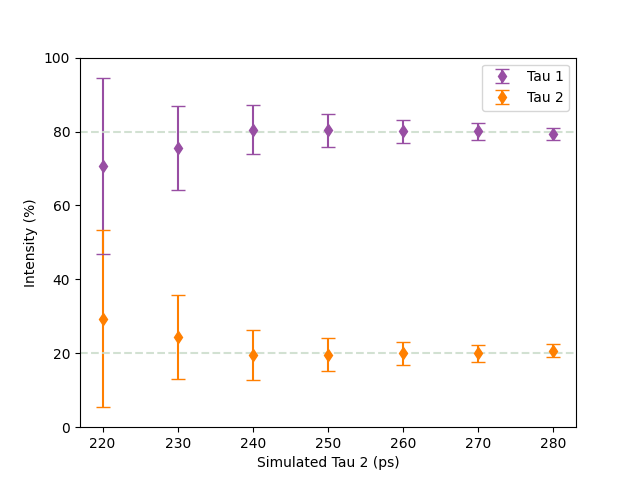
\includegraphics[width=0.95\linewidth]{Batch 1+2/8020.png}
        \caption{$\tau_1 = 80\%, \tau_2 = 20\%$}
        \label{fig:180-8020}
    \end{subfigure}
    }
\end{figure}

\pagebreak

\section{Modifying $\tau_1$}

A similar procedure was performed for $\tau_1$=150 and $\tau_1$=220. To keep the relative time interval the same in between batches, the corresponding spacing between $\tau_1$ and the $\tau_2$ range was kept consistent. For $\tau_1$ = 150, this meant a $\tau_2$ range of 190-250ps, and for $\tau_1$ = 220, this meant a corresponding $\tau_2$ range of 260-320ps.

This was first done for $\tau_1$ = 150. As can be seen in Figure \ref{fig:150}, the results for this batch are all within error, with both accuracy and precision getting better as the lifetime separation increases, in line with what would be expected.

The other batch, meanwhile, where $\tau_1$ was set to 220ps, was not as successful. The results can be seen in Figure \ref{fig:220}, but in general, PALSFIT struggled with fitting the lowest values for $\tau_2$ and the error bars are noticably larger. The program even gives nonsensical results when $\tau_1$ = 260ps and the relative $\tau_1$-$\tau_2$ intensity is set to 80\%-20\%, as can be seen in Figures \ref{fig:220-tau1}, \ref{fig:220-tau2} and \ref{fig:220-8020}.

In order to compare all three datasets, the absolute difference between the fitted and simulated values of each relevant variable, $\tau_1$, $\tau_2$ and intensity was plotted. Additionally, plots for their respective standard deviations were generated. The resulting plots are represented in Figures \ref{fig:t1-comp}-\ref{fig:int-comp}. Two general observations are apparent from analysis of these figures: 

The first is that the $\tau_2$ = 180ps data seems much more scattered than the other two datasets, which both follow a relatively clear increase in precision and accuracy as the lifetime separation increases. The second is that as $\tau_1$ decreases, PALSFIT seems better able to resolve the two lifetimes, with both the difference from the true value and the size of the error bars being the smallest when $\tau_1$ = 150ps.

\begin{figure}[p]
    \centering
    \caption{}
    \makebox[\linewidth][c]{
        \begin{subfigure}{0.7\textwidth}
        \centering
        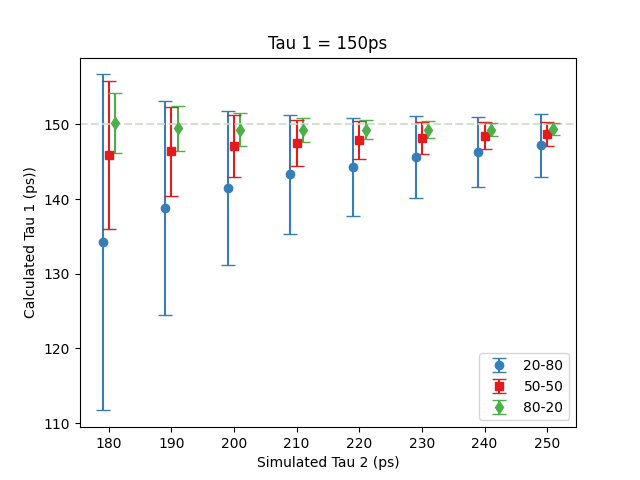
\includegraphics[width=0.95\linewidth]{Batch 3/regular IRF/tau1 150/output/t1.png}
        \caption{fixed $\tau_1 = 150ps$}
        \label{fig:150-tau1}
    \end{subfigure}
    \begin{subfigure}{0.7\textwidth}
        \centering
        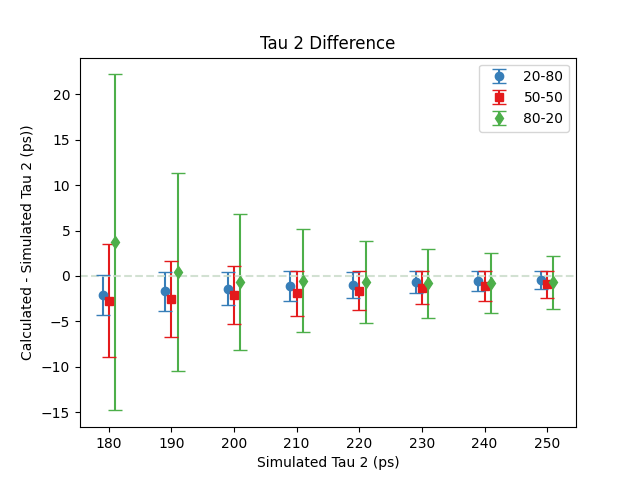
\includegraphics[width=.95\textwidth]{Batch 3/regular IRF/tau1 150/output/t2.png}
        \caption{$\tau_2$ difference}
        \label{fig:150-tau2}
    \end{subfigure}
    }
    \makebox[\linewidth][c]{
        \begin{subfigure}{0.7\textwidth}
        \centering
        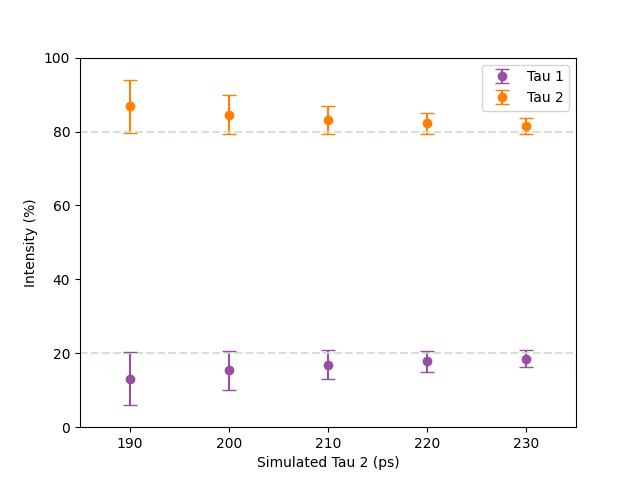
\includegraphics[width=0.95\linewidth]{Batch 3/regular IRF/tau1 150/output/2080r.png}
        \caption{$\tau_1 = 20\%, \tau_2 = 80\%$}
        \label{fig:150-2080}
    \end{subfigure}
    \begin{subfigure}{0.7\textwidth}
        \centering
        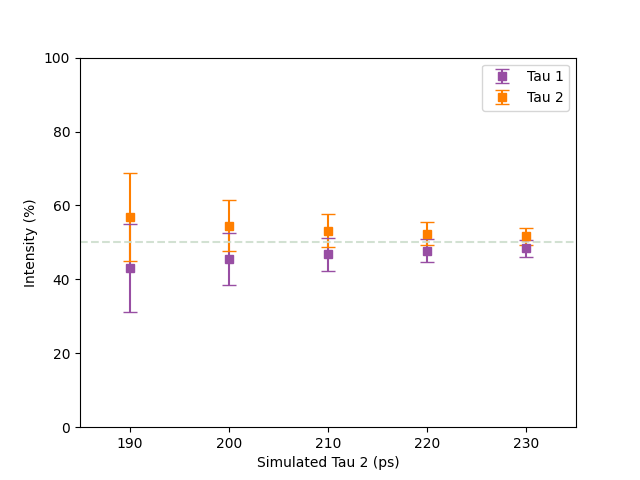
\includegraphics[width=.95\textwidth]{Batch 3/regular IRF/tau1 150/output/5050r.png}
        \caption{$\tau_1 = 50\%, \tau_2 = 50\%$}
        \label{fig:150-5050}
    \end{subfigure}
    }
    \begin{subfigure}{0.7\textwidth}
        \centering
        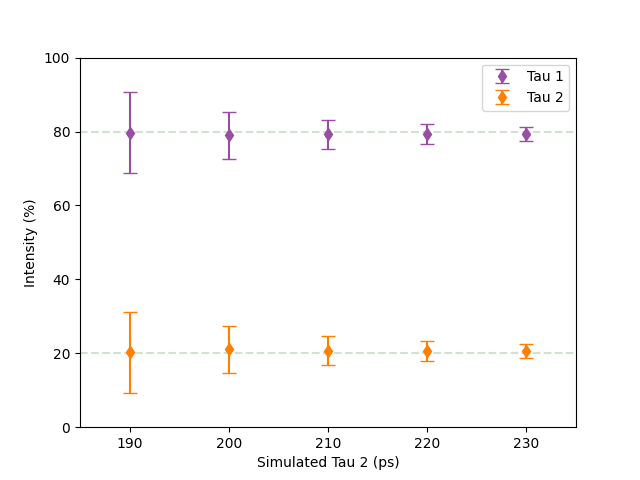
\includegraphics[width=.95\textwidth]{Batch 3/regular IRF/tau1 150/output/8020r.png}
        \caption{$\tau_1 = 80\%, \tau_2 = 20\%$}
        \label{fig:150-8020}
    \end{subfigure}
    \label{fig:150}
\end{figure}

\begin{figure}[p]
    \centering
    \caption{}
    \makebox[\linewidth][c]{
        \begin{subfigure}{0.7\textwidth}
        \centering
        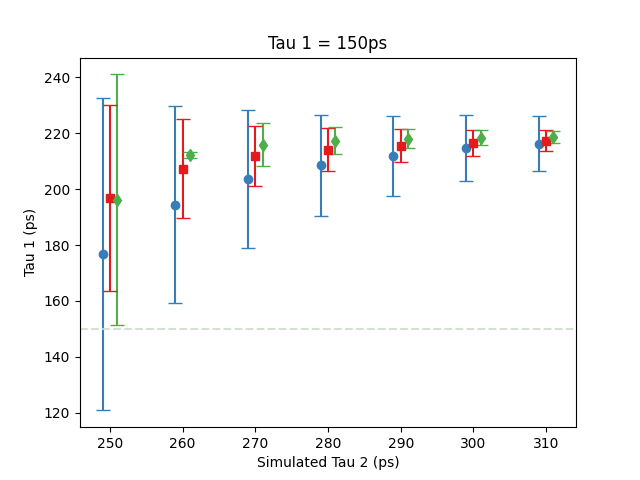
\includegraphics[width=0.95\linewidth]{Batch 3/regular IRF/tau1 220/output/t1.png}
        \caption{fixed $\tau_1 = 220ps$}
        \label{fig:220-tau1}
    \end{subfigure}
    \begin{subfigure}{0.7\textwidth}
        \centering
        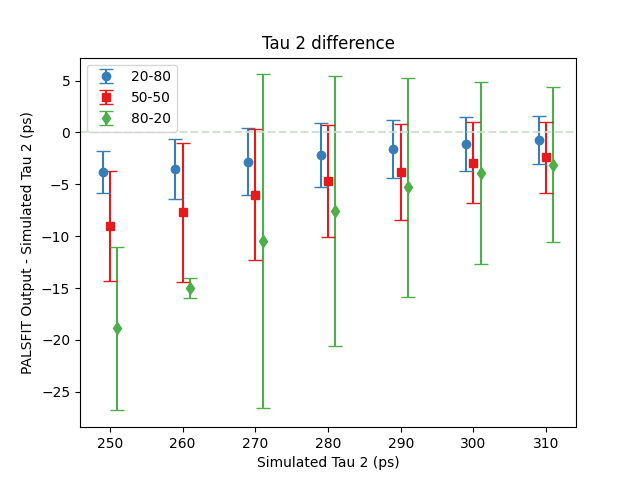
\includegraphics[width=.95\textwidth]{Batch 3/regular IRF/tau1 220/output/t2.png}
        \caption{$\tau_2$ difference}
        \label{fig:220-tau2}
    \end{subfigure}
    }
    \makebox[\linewidth][c]{
        \begin{subfigure}{0.7\textwidth}
        \centering
        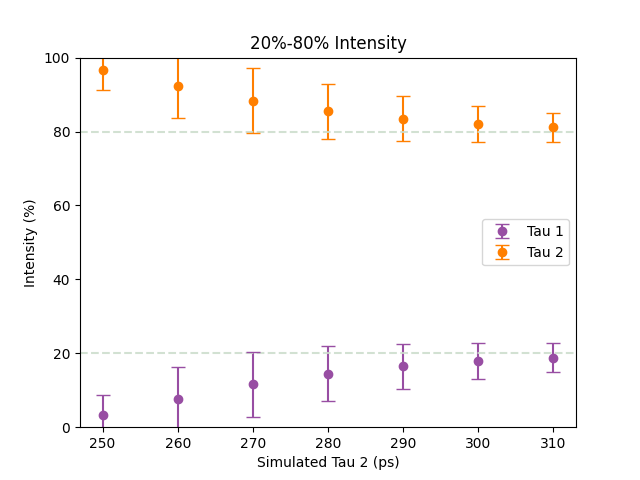
\includegraphics[width=0.95\linewidth]{Batch 3/regular IRF/tau1 220/output/2080.png}
        \caption{$\tau_1 = 20\%, \tau_2 = 80\%$}
        \label{fig:220-2080}
    \end{subfigure}
    \begin{subfigure}{0.7\textwidth}
        \centering
        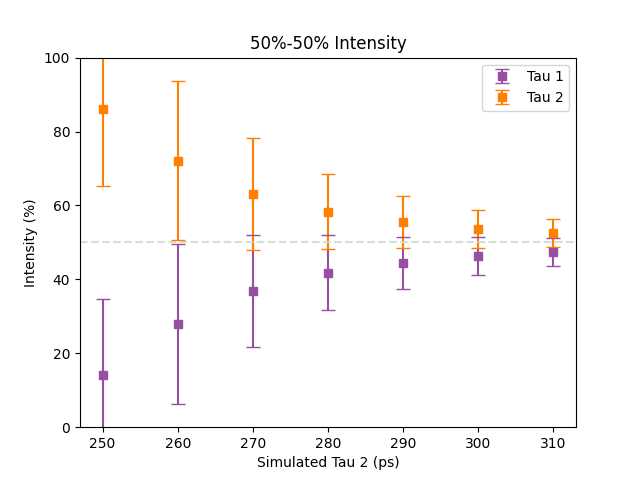
\includegraphics[width=.95\textwidth]{Batch 3/regular IRF/tau1 220/output/5050.png}
        \caption{$\tau_1 = 50\%, \tau_2 = 50\%$}
        \label{fig:220-5050}
    \end{subfigure}
    }
    \begin{subfigure}{0.7\textwidth}
        \centering
        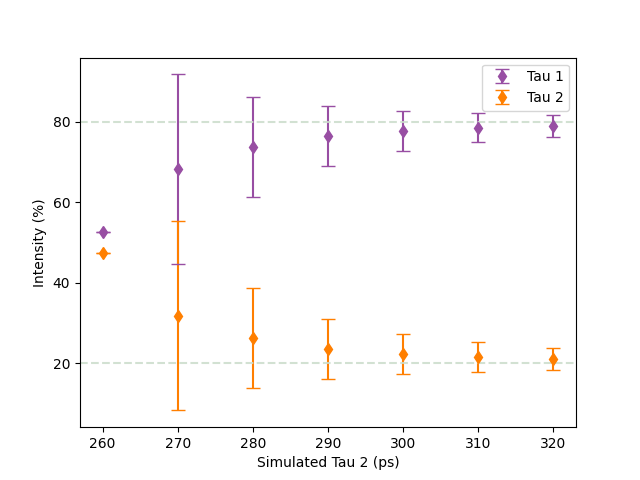
\includegraphics[width=.95\textwidth]{Batch 3/regular IRF/tau1 220/output/8020.png}
        \caption{$\tau_1 = 80\%, \tau_2 = 20\%$}
        \label{fig:220-8020}
    \end{subfigure}
    \label{fig:220}
\end{figure}

\begin{figure}[p]
    \centering
    \caption{$\tau_1$, rows = 20-80, 50-50, 80-20, columns = diff, std dev}    
    \makebox[\linewidth][c]{
        \begin{subfigure}{0.7\textwidth}
            \centering
            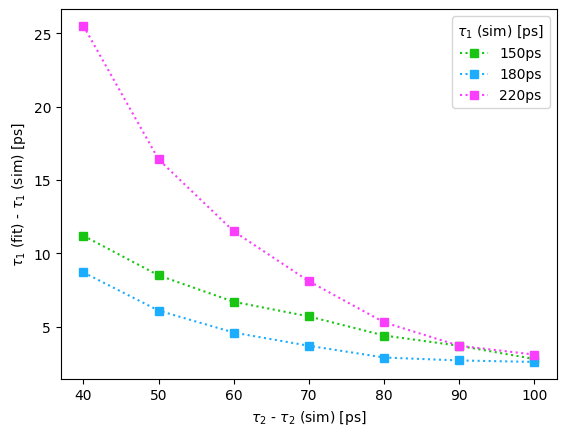
\includegraphics[width=0.95\linewidth]{Batch 3/regular IRF/t1-diff 2080.png}
            \label{fig:reg-t1-2080}
            \caption{}
        \end{subfigure}
        \begin{subfigure}{0.7\textwidth}
            \centering
            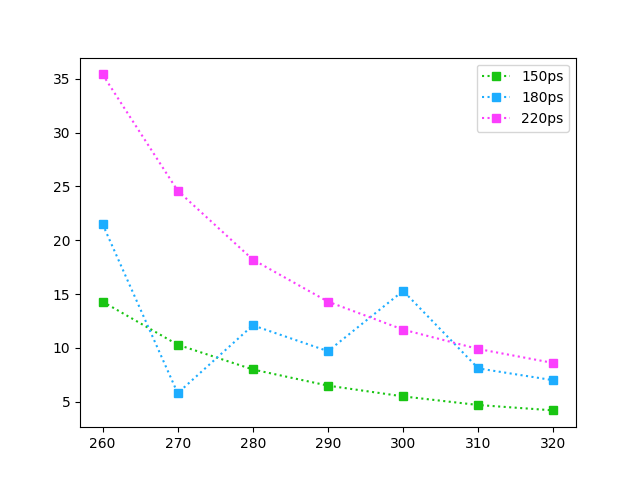
\includegraphics[width=0.95\linewidth]{Batch 3/regular IRF/t1-err 2080.png}
            \label{fig:reg-t1err-2080}
            \caption{}
        \end{subfigure}
    }

    \centering
    \makebox[\linewidth][c]{
        \begin{subfigure}{0.7\textwidth}
            \centering
            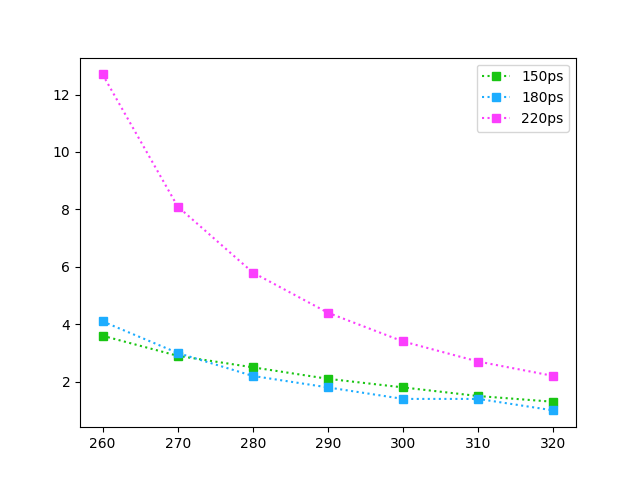
\includegraphics[width=0.95\linewidth]{Batch 3/regular IRF/t1-diff 5050.png}
            \label{fig:reg-t1-5050}
            \caption{}
        \end{subfigure}
        \begin{subfigure}{0.7\textwidth}
            \centering
            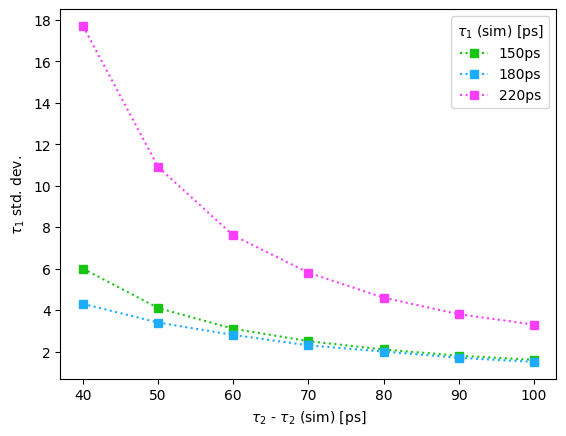
\includegraphics[width=0.95\linewidth]{Batch 3/regular IRF/t1-err 5050.png}
            \label{fig:reg-t1err-5050}
            \caption{}
        \end{subfigure}
    }

    \centering
    \makebox[\linewidth][c]{
        \begin{subfigure}{0.7\textwidth}
            \centering
            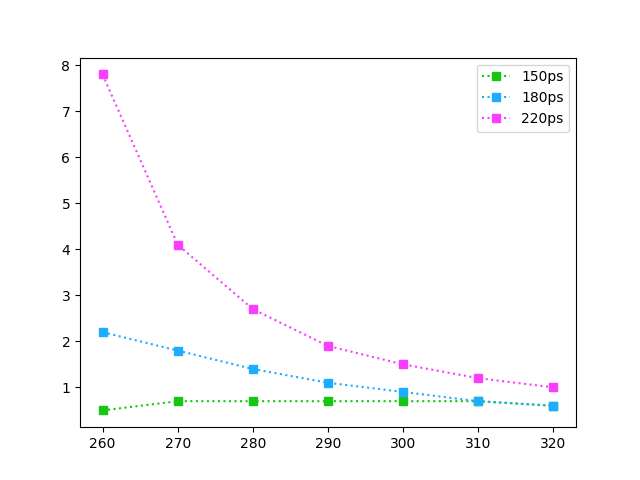
\includegraphics[width=0.95\linewidth]{Batch 3/regular IRF/t1-diff 8020.png}
            \label{fig:reg-t1-8020}
            \caption{}
        \end{subfigure}
        \begin{subfigure}{0.7\textwidth}
            \centering
            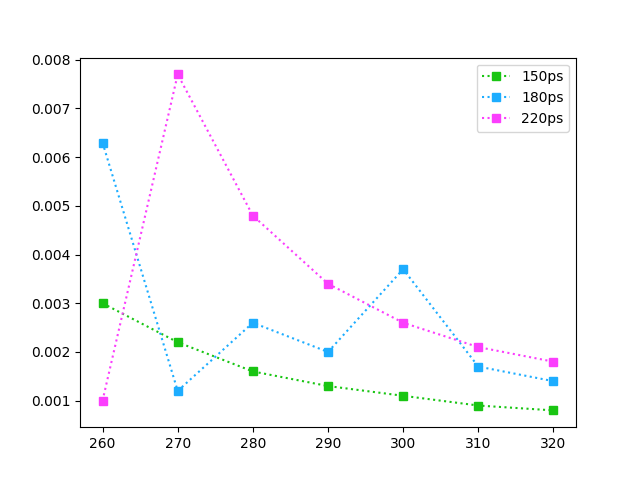
\includegraphics[width=0.95\linewidth]{Batch 3/regular IRF/t1-err 8020.png}
            \label{fig:reg-t1err-8020}
            \caption{}
        \end{subfigure}
    }

    \label{fig:t1-comp}
\end{figure}

\begin{figure}[p]
    \centering
    \caption{$\tau_2$, rows = 20-80, 50-50, 80-20, columns = diff, std dev}
    \makebox[\linewidth][c]{
        \begin{subfigure}{0.7\textwidth}
            \centering
            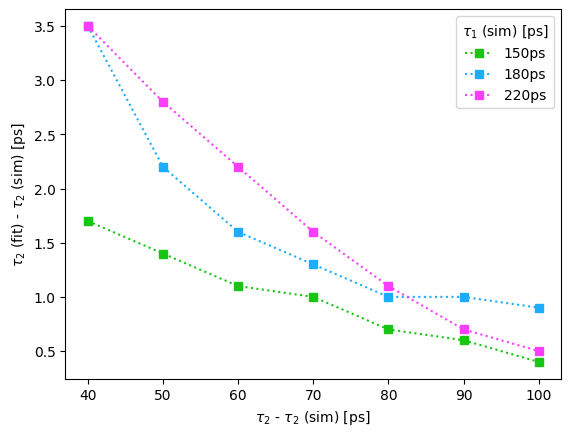
\includegraphics[width=0.95\linewidth]{Batch 3/regular IRF/t2-diff 2080.png}
            \label{fig:reg-t2-2080}
            \caption{}
        \end{subfigure}
        \begin{subfigure}{0.7\textwidth}
            \centering
            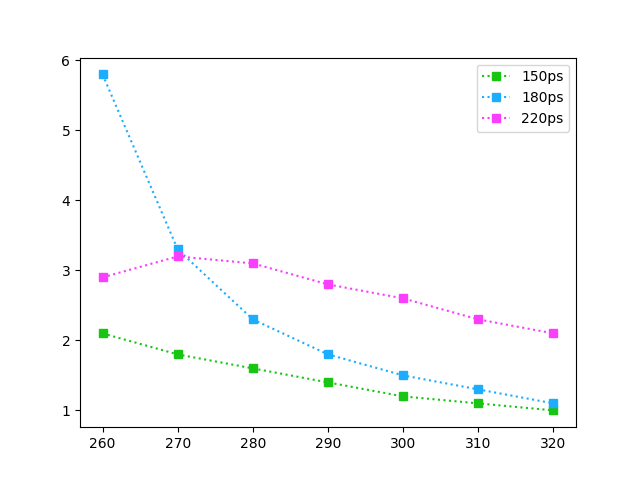
\includegraphics[width=0.95\linewidth]{Batch 3/regular IRF/t2-err 2080.png}
            \label{fig:reg-t2err-2080}
            \caption{}
        \end{subfigure}
    }

    \centering
    \makebox[\linewidth][c]{
        \begin{subfigure}{0.7\textwidth}
            \centering
            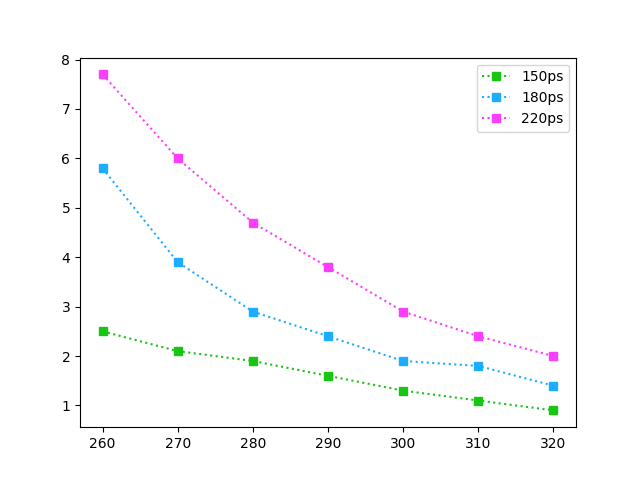
\includegraphics[width=0.95\linewidth]{Batch 3/regular IRF/t2-diff 5050.png}
            \label{fig:reg-t2-5050}
            \caption{}
        \end{subfigure}
        \begin{subfigure}{0.7\textwidth}
            \centering
            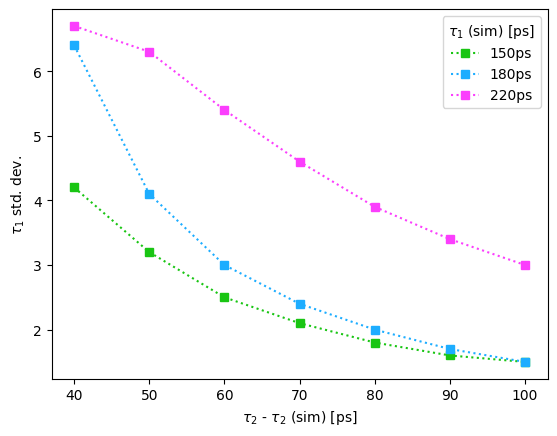
\includegraphics[width=0.95\linewidth]{Batch 3/regular IRF/t2-err 5050.png}
            \label{fig:reg-t2err-5050}
            \caption{}
        \end{subfigure}
    }

    \centering
    \makebox[\linewidth][c]{
        \begin{subfigure}{0.7\textwidth}
            \centering
            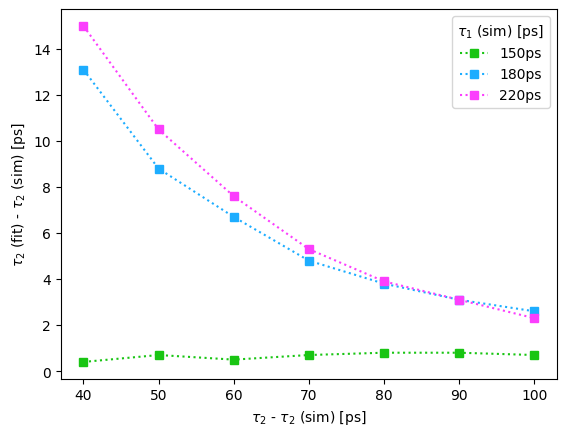
\includegraphics[width=0.95\linewidth]{Batch 3/regular IRF/t2-diff 8020.png}
            \label{fig:reg-t2-8020}
            \caption{}
        \end{subfigure}
        \begin{subfigure}{0.7\textwidth}
            \centering
            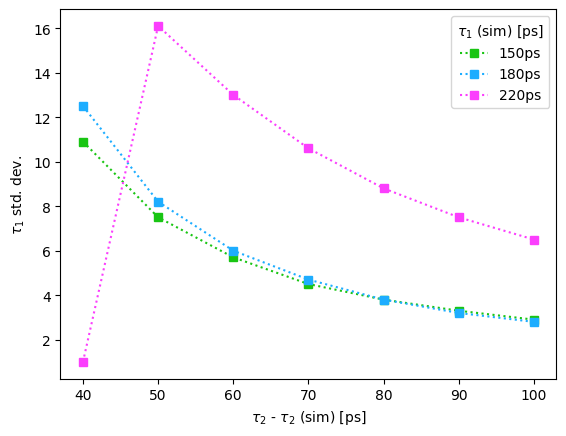
\includegraphics[width=0.95\linewidth]{Batch 3/regular IRF/t2-err 8020.png}
            \label{fig:reg-t2err-8020}
            \caption{}
        \end{subfigure}
    }
    
    \label{fig:t2-comp}
\end{figure}

\begin{figure}[p]
    \centering
    \caption{intensities, rows = 20-80, 50-50, 80-20, columns = diff, std dev}
    \makebox[\linewidth][c]{
        \begin{subfigure}{0.7\textwidth}
            \centering
            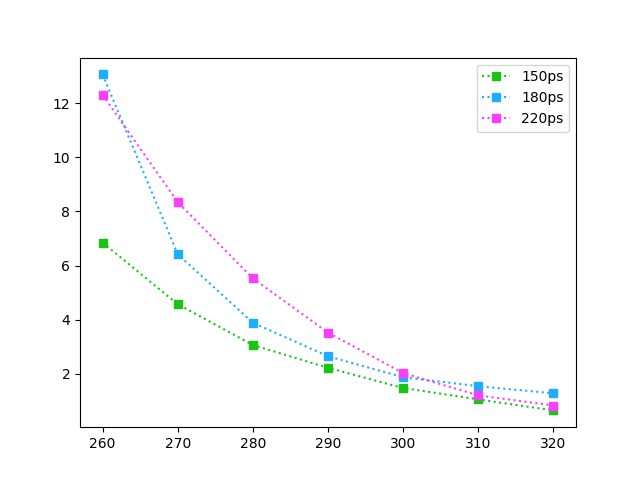
\includegraphics[width=0.95\linewidth]{Batch 3/regular IRF/2080-diff i1.png}
            \label{fig:reg-int-2080}
            \caption{}
        \end{subfigure}
        \begin{subfigure}{0.7\textwidth}
            \centering
            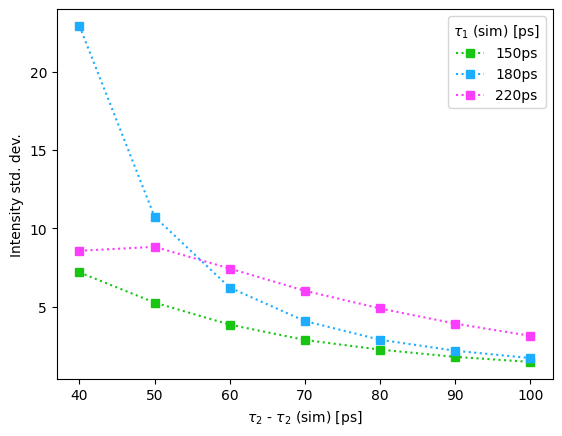
\includegraphics[width=0.95\linewidth]{Batch 3/regular IRF/2080-err i1.png}
            \label{fig:reg-interr-2080}
            \caption{}
        \end{subfigure}
    }

    \centering
    \makebox[\linewidth][c]{
        \begin{subfigure}{0.7\textwidth}
            \centering
            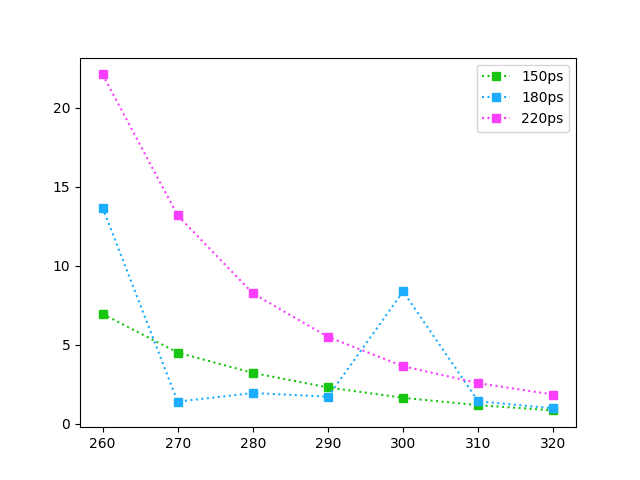
\includegraphics[width=0.95\linewidth]{Batch 3/regular IRF/5050-diff i1.png}
            \label{fig:reg-int-5050}
            \caption{}
        \end{subfigure}
        \begin{subfigure}{0.7\textwidth}
            \centering
            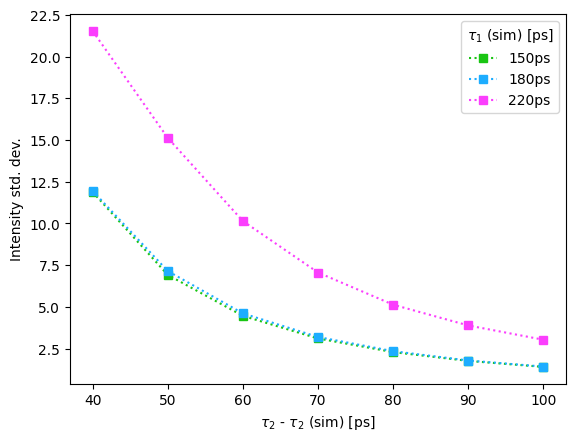
\includegraphics[width=0.95\linewidth]{Batch 3/regular IRF/5050-err i1.png}
            \label{fig:reg-interr-5050}
            \caption{}
        \end{subfigure}
    }

    \centering
    \makebox[\linewidth][c]{
        \begin{subfigure}{0.7\textwidth}
            \centering
            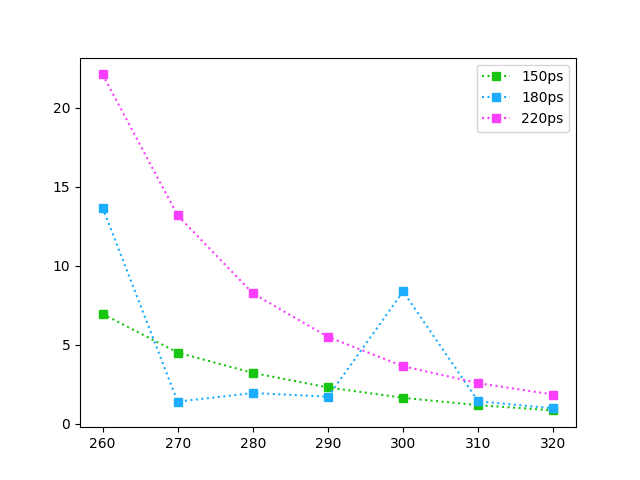
\includegraphics[width=0.95\linewidth]{Batch 3/regular IRF/5050-diff i1.png}
            \label{fig:reg-int-8020}
            \caption{}
        \end{subfigure}
        \begin{subfigure}{0.7\textwidth}
            \centering
            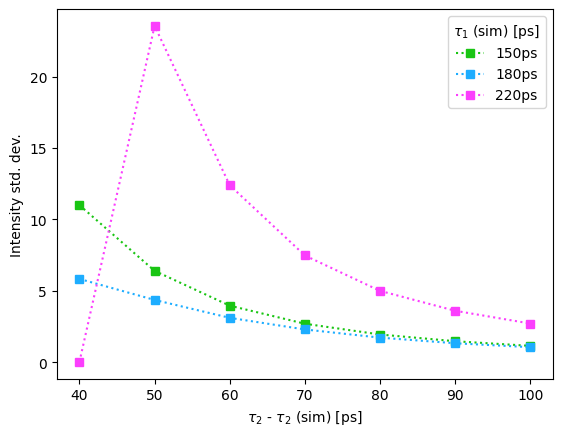
\includegraphics[width=0.95\linewidth]{Batch 3/regular IRF/8020-err i1.png}
            \label{fig:reg-interr-8020}
            \caption{}
        \end{subfigure}
    }
     
    \label{fig:int-comp}
\end{figure}

\pagebreak

\section{Single Gaussian IRF}

To investigate how the instrument resolution function affects the software, the three Gaussian resolution function in use so far can be simplified to a single Gaussian (refer to \dots) \todo{reference to justification, placed earlier}. As a sanity check, we can compare how the program 
performs with a single Gaussian resolution function versus the previous three Gaussian resolution function. Setting $\tau_1$ = 150ps, as this previously gave us the best results, we get the data in Figure \ref{fig:sing-210}. We can then compare this to Figure \ref{fig:150} and see that the single Gaussian resolution function produces remarkably similar results, demonstrating the single Gaussian approximation to be valid.

\begin{figure}[p]
    \centering
    \caption{}
    \makebox[\linewidth][c]{
        \begin{subfigure}{0.7\textwidth}
        \centering
        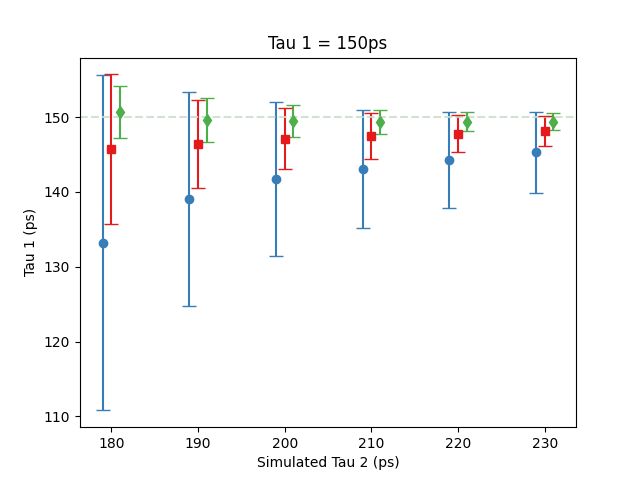
\includegraphics[width=0.95\linewidth]{Batch 3/single Gaussian IRF/gauss210/150/output/t1.png}
        \caption{fixed $\tau_1 = 150ps$}
        \label{fig:sing-210-tau1}
    \end{subfigure}
    \begin{subfigure}{0.7\textwidth}
        \centering
        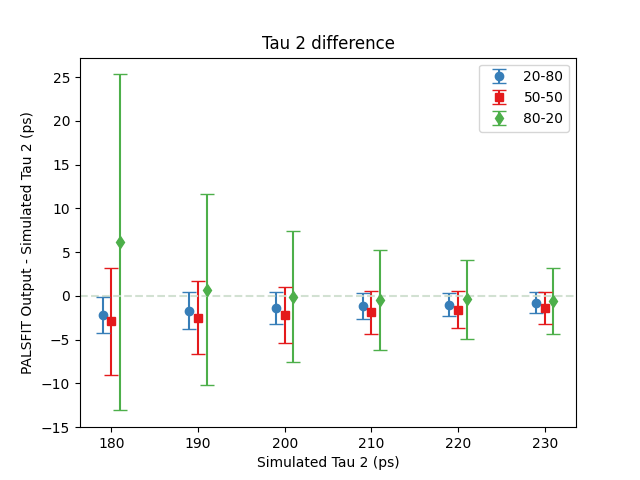
\includegraphics[width=.95\textwidth]{Batch 3/single Gaussian IRF/gauss210/150/output/t2.png}
        \caption{$\tau_2$ difference}
        \label{fig:sing-210-tau2}
    \end{subfigure}
    }
    \makebox[\linewidth][c]{
        \begin{subfigure}{0.7\textwidth}
        \centering
        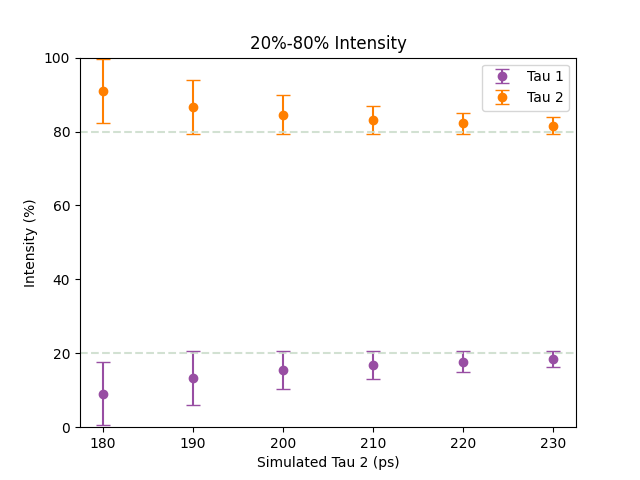
\includegraphics[width=0.95\linewidth]{Batch 3/single Gaussian IRF/gauss210/150/output/2080.png}
        \caption{$\tau_1 = 20\%, \tau_2 = 80\%$}
        \label{fig:sing-210-2080}
    \end{subfigure}
    \begin{subfigure}{0.7\textwidth}
        \centering
        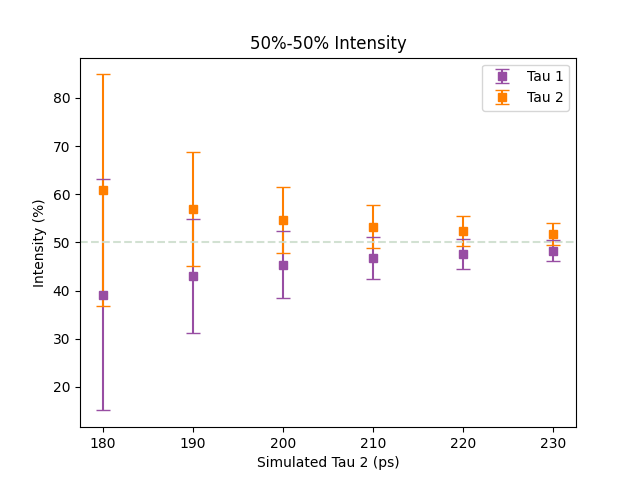
\includegraphics[width=.95\textwidth]{Batch 3/single Gaussian IRF/gauss210/150/output/5050.png}
        \caption{$\tau_1 = 50\%, \tau_2 = 50\%$}
        \label{fig:sing-210-5050}
    \end{subfigure}
    }
    \begin{subfigure}{0.7\textwidth}
        \centering
        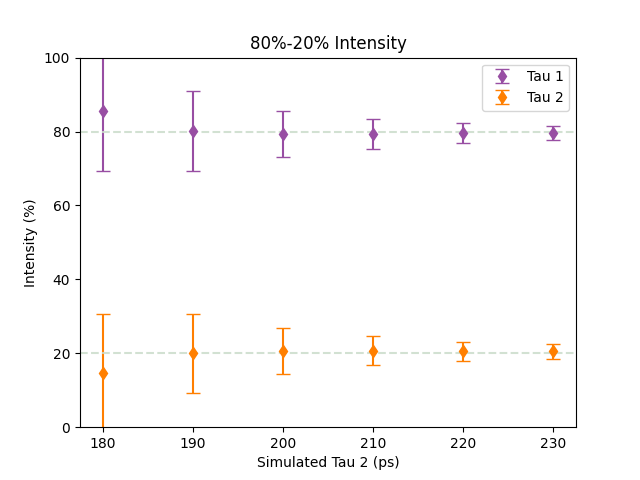
\includegraphics[width=.95\textwidth]{Batch 3/single Gaussian IRF/gauss210/150/output/8020.png}
        \caption{$\tau_1 = 80\%, \tau_2 = 20\%$}
        \label{fig:sing-210-8020}
    \end{subfigure}
    \label{fig:sing-210}
\end{figure}

With that established, spectra were generated and fitted for FWHM values of 220ps, 180ps, 150ps and 100ps, with $\tau_1$ set to 150ps and $\tau_2$ ranging from 180-230ps. In general, the trend we expect is the same increase in precision and accuracy with increasing $\tau_2$ that we see previously, but also an increase in both with narrower resolution functions. We would see this as multiple, separate, decreasing trendlines, ordered so that those corresponding to wider resolution functions were always higher. The results we get are shown in Figures \ref{fig:sing-t1-comp}-\ref{fig:sing-int-comp}, and we can analyse them in two parts.

If we just look at the subfigures on the left ((a),(c) and (e) for each figure), which represent the difference between the fit and original data, we see that for the 20\%-80\% and 50\%-50\% data the data follows the expected trend. When the $\tau_1$ intensity is set to \%80, however, we notice that accuracy doesn't seem to follow the expected relationship with the width of the resolution function. In many cases we have an outright reversal of the predicted relationship and in each figure we have significant crossing between the trendlines.

Looking at the subfigures on the right, representing the standard deviation of the fitting given by PALSFIT, we again see three outliers where the predicted relationship between precision and resolution function width is reversed, in Figures \ref{fig:sing-t2err-2080}, \ref{fig:sing-t2err-5050} and \ref{fig:sing-interr-2080}, though in the case of \ref{fig:sing-t2err-5050}, this reversed relationship quickly reverts to the expected one as $\tau_2$ increases.

\todo{
    possibly expand
}

\begin{figure}[p]
    \centering
    \caption{$\tau_1$, rows = 20-80, 50-50, 80-20, columns = diff, std dev}    
    \makebox[\linewidth][c]{
        \begin{subfigure}{0.7\textwidth}
            \centering
            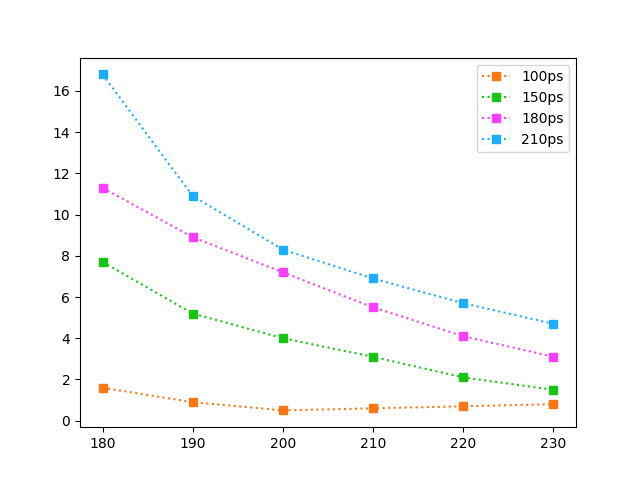
\includegraphics[width=0.95\linewidth]{Batch 3/single Gaussian IRF/t1-diff 2080.png}
            \caption{}
            \label{fig:sing-t1-2080}
        \end{subfigure}
        \begin{subfigure}{0.7\textwidth}
            \centering
            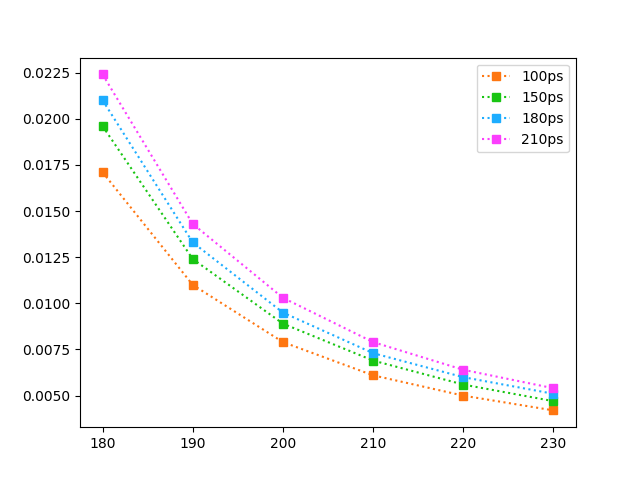
\includegraphics[width=0.95\linewidth]{Batch 3/single Gaussian IRF/t1-err 2080.png}
            \caption{}
            \label{fig:sing-t1err-2080}
        \end{subfigure}
    }

    \centering
    \makebox[\linewidth][c]{
        \begin{subfigure}{0.7\textwidth}
            \centering
            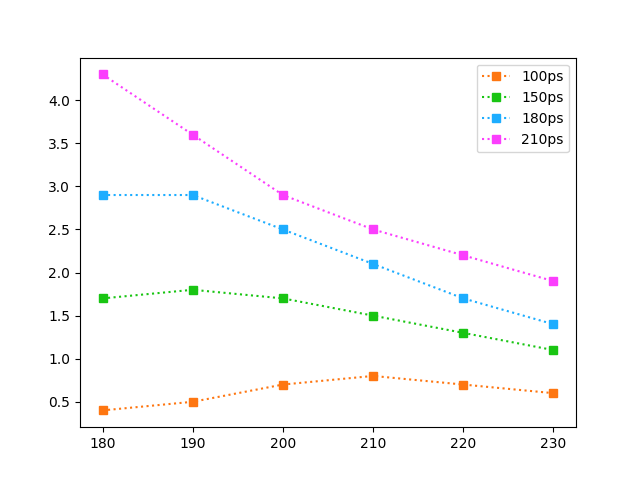
\includegraphics[width=0.95\linewidth]{Batch 3/single Gaussian IRF/t1-diff 5050.png}
            \caption{}
            \label{fig:sing-t1-5050}
        \end{subfigure}
        \begin{subfigure}{0.7\textwidth}
            \centering
            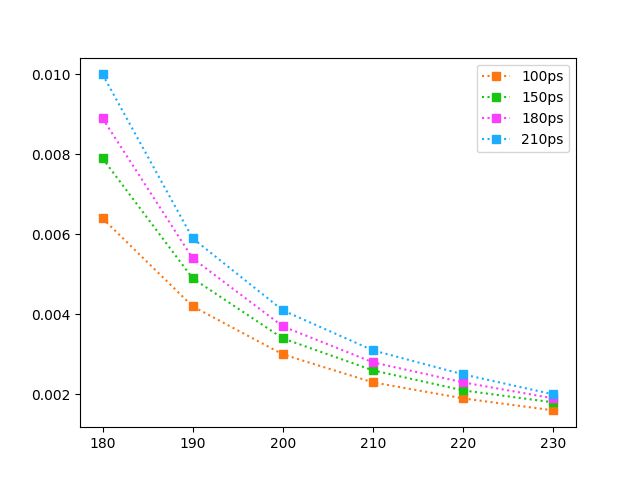
\includegraphics[width=0.95\linewidth]{Batch 3/single Gaussian IRF/t1-err 5050.png}
            \caption{}
            \label{fig:sing-t1err-5050}
        \end{subfigure}
    }

    \centering
    \makebox[\linewidth][c]{
        \begin{subfigure}{0.7\textwidth}
            \centering
            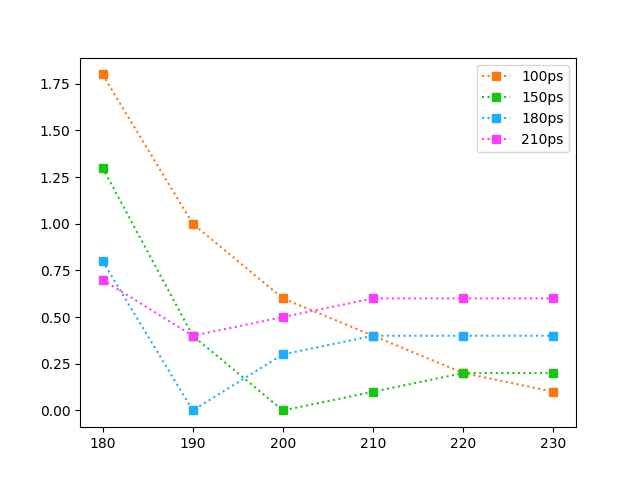
\includegraphics[width=0.95\linewidth]{Batch 3/single Gaussian IRF/t1-diff 8020.png}
            \caption{}
            \label{fig:sing-t1-8020}
        \end{subfigure}
        \begin{subfigure}{0.7\textwidth}
            \centering
            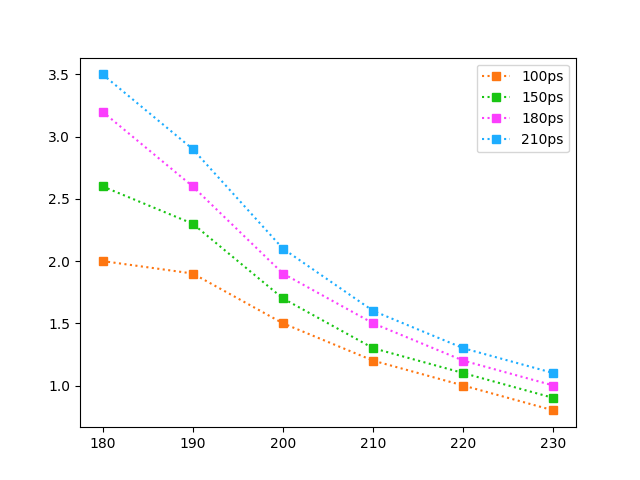
\includegraphics[width=0.95\linewidth]{Batch 3/single Gaussian IRF/t1-err 8020.png}
            \caption{}
            \label{fig:sing-t1err-8020}
        \end{subfigure}
    }

    \label{fig:sing-t1-comp}
\end{figure}

\begin{figure}[p]
    \centering
    \caption{$\tau_2$, rows = 20-80, 50-50, 80-20, columns = diff, std dev}
    \makebox[\linewidth][c]{
        \begin{subfigure}{0.7\textwidth}
            \centering
            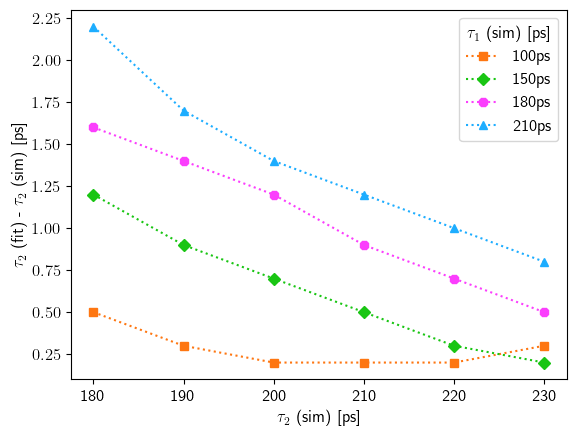
\includegraphics[width=0.95\linewidth]{Batch 3/single Gaussian IRF/t2-diff 2080.png}
            \caption{}
            \label{fig:sing-t2-2080}
        \end{subfigure}
        \begin{subfigure}{0.7\textwidth}
            \centering
            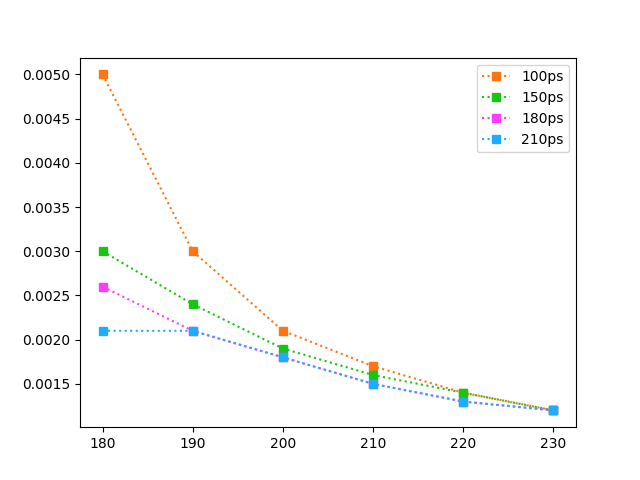
\includegraphics[width=0.95\linewidth]{Batch 3/single Gaussian IRF/t2-err 2080.png}
            \caption{}
            \label{fig:sing-t2err-2080}
        \end{subfigure}
    }

    \centering
    \makebox[\linewidth][c]{
        \begin{subfigure}{0.7\textwidth}
            \centering
            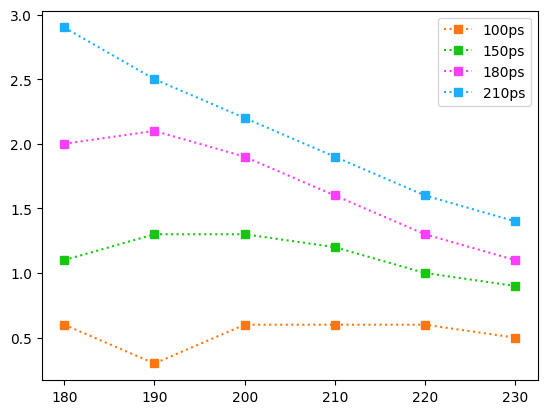
\includegraphics[width=0.95\linewidth]{Batch 3/single Gaussian IRF/t2-diff 5050.png}
            \caption{}
            \label{fig:sing-t2-5050}
        \end{subfigure}
        \begin{subfigure}{0.7\textwidth}
            \centering
            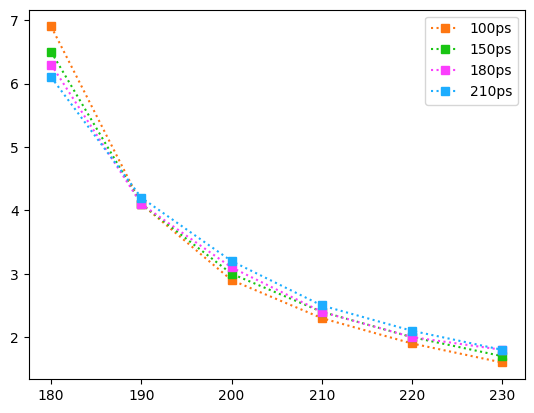
\includegraphics[width=0.95\linewidth]{Batch 3/single Gaussian IRF/t2-err 5050.png}
            \caption{}
            \label{fig:sing-t2err-5050}
        \end{subfigure}
    }

    \centering
    \makebox[\linewidth][c]{
        \begin{subfigure}{0.7\textwidth}
            \centering
            \includegraphics[width=0.95\linewidth]{Batch 3/single Gaussian IRF/t2-diff 8020.png}
            \caption{}
            \label{fig:sing-t2-8020}
        \end{subfigure}
        \begin{subfigure}{0.7\textwidth}
            \centering
            \includegraphics[width=0.95\linewidth]{Batch 3/single Gaussian IRF/t2-err 8020.png}
            \caption{}
            \label{fig:sing-t2err-8020}
        \end{subfigure}
    }
    
    \label{fig:sing-t2-comp}
\end{figure}

\begin{figure}[p]
    \centering
    \caption{intensities, rows = 20-80, 50-50, 80-20, columns = diff, std dev}
    \makebox[\linewidth][c]{
        \begin{subfigure}{0.7\textwidth}
            \centering
            \includegraphics[width=0.95\linewidth]{Batch 3/single Gaussian IRF/2080-diff i1.png}
            \caption{}
            \label{fig:sing-int-2080}
        \end{subfigure}
        \begin{subfigure}{0.7\textwidth}
            \centering
            \includegraphics[width=0.95\linewidth]{Batch 3/single Gaussian IRF/2080-err i1.png}
            \caption{}
            \label{fig:sing-interr-2080}
        \end{subfigure}
    }

    \centering
    \makebox[\linewidth][c]{
        \begin{subfigure}{0.7\textwidth}
            \centering
            \includegraphics[width=0.95\linewidth]{Batch 3/single Gaussian IRF/5050-diff i1.png}
            \caption{}
            \label{fig:sing-int-5050}
        \end{subfigure}
        \begin{subfigure}{0.7\textwidth}
            \centering
            \includegraphics[width=0.95\linewidth]{Batch 3/single Gaussian IRF/5050-err i1.png}
            \caption{}
            \label{fig:sing-interr-5050}
        \end{subfigure}
    }

    \centering
    \makebox[\linewidth][c]{
        \begin{subfigure}{0.7\textwidth}
            \centering
            \includegraphics[width=0.95\linewidth]{Batch 3/single Gaussian IRF/8020-diff i1.png}
            \caption{}
            \label{fig:sing-int-8020}
        \end{subfigure}
        \begin{subfigure}{0.7\textwidth}
            \centering
            \includegraphics[width=0.95\linewidth]{Batch 3/single Gaussian IRF/8020-err i1.png}
            \caption{}
            \label{fig:sing-interr-8020}
        \end{subfigure}
    }
     
    \label{fig:sing-int-comp}
\end{figure}

\pagebreak

\section{Number of counts}

Another variable worth examining is the total number of counts in a given spectrum. When generating spectra using PALSSIM, this is given as the area of the spectrum without the background and a separate background value. Both were kept constant in all previous runs, with the area set to $5.65 \times 10^6$ and the background value set to 8.5. Expectations are that a higher number of counts would make spectrum analysis easier. To test this hypothesis, spectra with generated for $\tau_1$ = 150ps, $\tau_2$ = 180-230ps and a 210ps FWHM single gaussian resolution function, tripling the background area to $1.7035 \times 10^7$.

If we just increase the total area of the spectra and maintain the same background value as before, however, we inadvertently end up increasing the signal to noise ratio. While this would be desirable, in a practical setting an increase in total number of counts most likely corresponds to an increase in background noise. As such, spectra were also generated with both the tripled area and a proportional 3x increase in the background value (set to 25.5).

The generated spectra were then analyzed with PALSFIT, and the results are summarized in Figures \ref{fig:bg-t1-comp}-\ref{fig:bg-int-comp}, with a "regular" run for comparison. The regular run is simply the one represented in Figure \ref{fig:sing-210}, which used the original, unaltered area and background value.

Looking first at the standard deviations (subfigures (b), (d) and (f), on the right side of the page), we see that, as expected, the data from the regular run is in most cases significantly less precise than the other two runs. Additionally, the data with the proportionally scaled background value seems to be slightly less precise than its unscaled counterpart, though in many cases just barely so, if at all. Exceptions tend to occur, however, for the shortest lifetime separation, when $\tau_2$ is set to 180ps.

Looking at the left side of the figures ((a), (c) and (e)), we see that for the most part the first trend seem to hold true, with the regular run being significantly less accurate than the other two. The exception to this seems to be when the relative $\tau_1$-$\tau_2$ intensity is 80\%-20\%, in which we often have a reversal of expectations, at times with some significant crossover of the relevant trendlines. While, at a glance, the normal and scaled background triple area runs are still for the most part relatively close, with the proportional background looking less accurate overall, this isn't as universally true as it is when looking at the standard deviation. Specifically in Figures \ref{fig:bg-t1-2080}, \ref{fig:bg-t2-2080} and \ref{fig:bg-int-2080}, when $\tau_1$ = 20\% and $\tau_2$ = 80\%, PALSFIT seems to have performed worse with the non-scaled background, at least for significant portions of the graphs.

\begin{figure}[p]
    \centering
    \caption{$\tau_1$, rows = 20-80, 50-50, 80-20, columns = diff, std dev}    
    \makebox[\linewidth][c]{
        \begin{subfigure}{0.7\textwidth}
            \centering
            \includegraphics[width=0.95\linewidth]{Batch 5/t1-diff 2080.png}
            \caption{}
            \label{fig:bg-t1-2080}
        \end{subfigure}
        \begin{subfigure}{0.7\textwidth}
            \centering
            \includegraphics[width=0.95\linewidth]{Batch 5/t1-err 2080.png}
            \caption{}
            \label{fig:bg-t1err-2080}
        \end{subfigure}
    }

    \centering
    \makebox[\linewidth][c]{
        \begin{subfigure}{0.7\textwidth}
            \centering
            \includegraphics[width=0.95\linewidth]{Batch 5/t1-diff 5050.png}
            \caption{}
            \label{fig:bg-t1-5050}
        \end{subfigure}
        \begin{subfigure}{0.7\textwidth}
            \centering
            \includegraphics[width=0.95\linewidth]{Batch 5/t1-err 5050.png}
            \caption{}
            \label{fig:bg-t1err-5050}
        \end{subfigure}
    }

    \centering
    \makebox[\linewidth][c]{
        \begin{subfigure}{0.7\textwidth}
            \centering
            \includegraphics[width=0.95\linewidth]{Batch 5/t1-diff 8020.png}
            \caption{}
            \label{fig:bg-t1-8020}
        \end{subfigure}
        \begin{subfigure}{0.7\textwidth}
            \centering
            \includegraphics[width=0.95\linewidth]{Batch 5/t1-err 8020.png}
            \caption{}
            \label{fig:bg-t1err-8020}
        \end{subfigure}
    }

    \label{fig:bg-t1-comp}
\end{figure}

\begin{figure}[p]
    \centering
    \caption{$\tau_2$, rows = 20-80, 50-50, 80-20, columns = diff, std dev}
    \makebox[\linewidth][c]{
        \begin{subfigure}{0.7\textwidth}
            \centering
            \includegraphics[width=0.95\linewidth]{Batch 5/t2-diff 2080.png}
            \caption{}
            \label{fig:bg-t2-2080}
        \end{subfigure}
        \begin{subfigure}{0.7\textwidth}
            \centering
            \includegraphics[width=0.95\linewidth]{Batch 5/t2-err 2080.png}
            \caption{}
            \label{fig:bg-t2err-2080}
        \end{subfigure}
    }

    \centering
    \makebox[\linewidth][c]{
        \begin{subfigure}{0.7\textwidth}
            \centering
            \includegraphics[width=0.95\linewidth]{Batch 5/t2-diff 5050.png}
            \caption{}
            \label{fig:bg-t2-5050}
        \end{subfigure}
        \begin{subfigure}{0.7\textwidth}
            \centering
            \includegraphics[width=0.95\linewidth]{Batch 5/t2-err 5050.png}
            \caption{}
            \label{fig:bg-t2err-5050}
        \end{subfigure}
    }

    \centering
    \makebox[\linewidth][c]{
        \begin{subfigure}{0.7\textwidth}
            \centering
            \includegraphics[width=0.95\linewidth]{Batch 5/t2-diff 8020.png}
            \caption{}
            \label{fig:bg-t2-8020}
        \end{subfigure}
        \begin{subfigure}{0.7\textwidth}
            \centering
            \includegraphics[width=0.95\linewidth]{Batch 5/t2-err 8020.png}
            \caption{}
            \label{fig:bg-t2err-8020}
        \end{subfigure}
    }
    
    \label{fig:bg-t2-comp}
\end{figure}

\begin{figure}[p]
    \centering
    \caption{intensities, rows = 20-80, 50-50, 80-20, columns = diff, std dev}
    \makebox[\linewidth][c]{
        \begin{subfigure}{0.7\textwidth}
            \centering
            \includegraphics[width=0.95\linewidth]{Batch 5/2080-diff i1.png}
            \caption{}
            \label{fig:bg-int-2080}
        \end{subfigure}
        \begin{subfigure}{0.7\textwidth}
            \centering
            \includegraphics[width=0.95\linewidth]{Batch 5/2080-err i1.png}
            \caption{}
            \label{fig:bg-interr-2080}
        \end{subfigure}
    }

    \centering
    \makebox[\linewidth][c]{
        \begin{subfigure}{0.7\textwidth}
            \centering
            \includegraphics[width=0.95\linewidth]{Batch 5/5050-diff i1.png}
            \caption{}
            \label{fig:bg-int-5050}
        \end{subfigure}
        \begin{subfigure}{0.7\textwidth}
            \centering
            \includegraphics[width=0.95\linewidth]{Batch 5/5050-err i1.png}
            \caption{}
            \label{fig:bg-interr-5050}
        \end{subfigure}
    }

    \centering
    \makebox[\linewidth][c]{
        \begin{subfigure}{0.7\textwidth}
            \centering
            \includegraphics[width=0.95\linewidth]{Batch 5/8020-diff i1.png}
            \caption{}
            \label{fig:bg-int-8020}
        \end{subfigure}
        \begin{subfigure}{0.7\textwidth}
            \centering
            \includegraphics[width=0.95\linewidth]{Batch 5/8020-err i1.png}
            \caption{}
            \label{fig:bg-interr-8020}
        \end{subfigure}
    }
     
    \label{fig:bg-int-comp}
\end{figure}

\pagebreak


\iffalse

Using Python, we can plot the three gaussian functions that compose the instrument resolution function. The equation for a Gaussian function with parameters $a$, $b$ and $c$ (corresponding to the height of the peak, the position of the peak and the width of the graph) is given by the equation:

\[g(x) = a\exp{\left(-\frac{(x-b)^2}{2c^2}\right)} \]

While $a$ and $b$ map easily to the intensity and shift columns in Table \ref{tab:irf} ,  $c$ is expressed as a standard deviation, and not the full-half-width-maximum given in the table. To convert from one to the other, we can use the following expression:

\[ FWHM = 2\sqrt{2\ln(2)} \approx 2.355c \]

The resultant resolution function is, then, just the sum of the three gaussians $g_s(x)$, where

\[g_s(x) = \sum_{i=1}^{3}{a_i \exp{\left(-\frac{(x-b)^2}{2c^2}\right)}}\]

This resolution function looks quite similar to a gaussian function itself, and thus it seems sensible to investigate the feasability of approximating a more complex 3 gaussian resolution function, with a single gaussian.

The intensity of the single gaussian approximation is the easiest parameter to determine, as it's simply 100\%. We could try to determine $b$ and $c$ analytically by solving the resulting $g_s(x)$ analytically, but, as we already have already generated a list of values for $g_s(x)$ when plotting the function, it's much easier to just extract the needed values numerically using Python.

Finding $b$ is as easy as finding the largest element of the list, and its corresponding $x$ value. As PALSSIM requires the FWHM rather than the standard deviation $c$, we just need to find the difference between the two values of $x$ for which $g_s(x)$ is closest to half of the IRF.

Doing so gives us the following values to insert into PALSSIM:

\begin{table}[h]
    \centering
    \begin{tabular}{|c|c|c|}
        \hline
        FWHM (ps) &  Shift (ps) & Intensity (\%) \\
        \hline
        210 & 0 & 100\\ 
        \hline
    \end{tabular}
    \caption{Single gaussian Instrument resolution function}
    \label{tab:irf-single}
\end{table}

Plugging in these values into PALSSIM gives us very similar results to the three gaussian IRF, with slight differences in the first datapoint for some of the graphs. Overall, though, it does seems like we can reasonably approximate a more complex, three gaussian IRF with a single gaussian.

The next step would be to examine how the width of the instrument resolution function (IRF) affects the results. The values for $\tau_1$ and $\tau_2$ can be set to be kept the same between runs, with $\tau_1$ fixed to 150ps and $\tau_2$ ranging from 180-230ps, as we had the best results with these values. The full-width half maximum of our single gaussian IRF can be set to the following values: 100ps, 150ps, 180ps, 210ps.

\fi


\section{Realistic data}

Analysis of real world data often differs from how we've conducted our analysis so far. One key factor is that usually the number of lifetimes present in a real life spectrum isn't known beforehand. As PALSFIT requires the user to input the number of fitted lifetimes, this might lead to situations in which the user predicts the wrong number of lifetimes, thus it might be useful to explore how the software behaves in such a situation.

To do so, three materials (?) were modeled, with three lifetime components. All three have two shorter components that differed between them, and a long lifetime component set to 2.6ns with a 0.15\% intensity that was kept equal. The relative intensities of the two shorter lifetime components were adjusted to the following values:

\begin{table}[h]
    \centering
    \begin{subtable}[t]{0.48\textwidth}
        \flushleft
        \begin{tabular}{|c|c|c|c|}
            \hline
            \multicolumn{2}{|c|}{relative} & \multicolumn{2}{|c|}{absolute} \\
            \hline
            $\tau_1$ & $\tau_2$ & $\tau_1$    & $\tau_2$   \\
            \hline
            99.5\% & 0.5\% & 99.3508\%*  &  0.4993\%* \\
            90\%   & 10\% & 89.865\%    &  9.985\%   \\
            80\%   & 20\% & 89.88\%     & 19.97\%    \\
            50\%   & 50\% & 49.925\%    & 49.925\%   \\
            20\%   & 80\% & 19.97\%     &  9.985\%   \\
            \hline
        \end{tabular}
        \caption{intensities}
    \end{subtable}

    \hspace{\fill}

    \begin{subtable}[t]{0.48\textwidth}
        \begin{tabular}{|c|c|c|}
            \hline
            $\tau_1$(ps) & $\tau_2$(ps) & $\tau_3$(ns)\\
            \hline
            370 & 442 & 2.6 \\
            355 & 444 & 2.6 \\
            348 & 440 & 2.6 \\
            \hline
        \end{tabular}
        \caption{lifetimes}
    \end{subtable}
\end{table}

When a single lifetime is fitted, the resulting lifetime seems to tend towards a weighted average of the two shorter lifetimes, as can be seen in the following figures:

\begin{figure}[p]
    \centering
    \makebox[\linewidth][c]{
        \begin{subfigure}{0.7\textwidth}
            \centering
            \includegraphics[width=0.95\linewidth]{Batch 6/1-life/lifetime.png}
            \caption{$\tau_1$ = 370, $\tau_2$ = 442}
            \label{fig:1life_370}
        \end{subfigure}
        \begin{subfigure}{0.7\textwidth}
            \centering
            \includegraphics[width=0.95\linewidth]{Batch 7/355-444/output/1 life/lifetime.png}
            \caption{$\tau_1$ = 355, $\tau_2$ = 444}
            \label{fig:1life-355}
        \end{subfigure}
    }
    \centering
    \makebox[\linewidth][c]{
        \begin{subfigure}{0.7\textwidth}
            \centering
            \includegraphics[width=0.95\linewidth]{Batch 7/348-440/output/1 life/lifetime.png}
            \caption{$\tau_1$ = 348, $\tau_2$ = 440}
            \label{fig:1life_348}
        \end{subfigure}
    }
    \label{fig:1life}
    \caption{single lifetime fit} 
\end{figure}

\begin{figure}[p]
    \centering
    \makebox[\linewidth][c]{
        \begin{subfigure}{0.7\textwidth}
            \centering
            \includegraphics[width=0.95\linewidth]{Batch 6/2-life/lifetimes.png}
            \caption{$\tau_1$ = 370, $\tau_2$ = 442}
            \label{fig:2life_370}
        \end{subfigure}
        \begin{subfigure}{0.7\textwidth}
            \centering
            \includegraphics[width=0.95\linewidth]{Batch 7/355-444/output/2 life/lifetimes.png}
            \caption{$\tau_1$ = 355, $\tau_2$ = 444}
            \label{fig:2life-355}
        \end{subfigure}
    }
    \centering
    \makebox[\linewidth][c]{
        \begin{subfigure}{0.7\textwidth}
            \centering
            \includegraphics[width=0.95\linewidth]{Batch 7/348-440/output/2 life/lifetimes.png}
            \caption{$\tau_1$ = 348, $\tau_2$ = 440}
            \label{fig:2life_348}
        \end{subfigure}
    }
    \label{fig:2life}
    \caption{two lifetime fit} 
\end{figure}

\begin{figure}[p]
    \centering
    \makebox[\linewidth][c]{
        \begin{subfigure}{0.7\textwidth}
            \centering
            \includegraphics[width=0.95\linewidth]{Batch 6/3-life/lifetimes.png}
            \caption{$\tau_1$ = 370, $\tau_2$ = 442}
            \label{fig:3life_370}
        \end{subfigure}
        \begin{subfigure}{0.7\textwidth}
            \centering
            \includegraphics[width=0.95\linewidth]{Batch 7/355-444/output/3 life/lifetimes.png}
            \caption{$\tau_1$ = 355, $\tau_2$ = 444}
            \label{fig:3life-355}
        \end{subfigure}
    }
    \centering
    \makebox[\linewidth][c]{
        \begin{subfigure}{0.7\textwidth}
            \centering
            \includegraphics[width=0.95\linewidth]{Batch 7/348-440/output/3 life/lifetimes.png}
            \caption{$\tau_1$ = 348, $\tau_2$ = 440}
            \label{fig:3life_348}
        \end{subfigure}
    }
    \label{fig:3life}
    \caption{three lifetime fit} 
\end{figure}